\documentclass[handout, aspectratio=169]{beamer}
\mode<presentation>{}
\usepackage[utf8]{inputenc}
\newcommand{\fl}[1]{\left\lfloor #1 \right\rfloor}
\usepackage{tikz}

\title{MA 105 : Calculus\\ D1 - T5, Tutorial 12}  % change
\author{Aryaman Maithani}
\date[23-10-2019]{23rd October, 2019}               % change
\institute[IITB]{IIT Bombay}
\usetheme{Warsaw}
\usecolortheme{beetle}
\newtheorem{defn}{Definition}
\begin{document}
\begin{frame}
	\titlepage
\end{frame}
\begin{frame}{Sheet 9}                            % change
	(7) We know that the line integral of a continuous scalar field along a smooth is independent of the parameterisation. The question given indeed does satisfy these conditions. Hence, we may choose any parameterisation of our choice.\\
	\uncover<2->{Let $c:[-1, 1] \to \mathbb{R}^2$ be defined as $c(t) := (t, t^2).$ }\\
	\uncover<3->{Then, the required line is integral is given as }\\
	\uncover<4->{\[\int_{-1}^{1} \mathbf{f}(c(t))\cdot c'(t) dt .\] }\\
	\uncover<5->{We compute $c'(t) = (1, 2t).$ }\\
	\uncover<6->{\[\text{Thus,} \int_{-1}^{1} \mathbf{f}(c(t))\cdot c'(t) dt = \int_{-1}^{1} (2t^5 - 4t^4 - 2t^3 + t^2) dt \] }
	\uncover<-7>{\[= -\frac{14}{15}\] }
\end{frame}
\begin{frame}{Sheet 9}
	(9) Let us parameterise the curve $C$ as $c(t) := \left(x(t), y(t)\right) := (a\cos t, a\sin t)$ for $t \in [-\pi, \pi].$\\
	\uncover<2->{Note that this does parameterise the curve in the desired direction. }\\
	\uncover<3->{With this parameterisation, we now get: }
	\uncover<4->{\[\oint_C \frac{x+y}{x^2 + y^2}dx = \int_{-\pi}^{\pi} \left(\frac{\cos t + \sin t}{a}\right)x'(t) dt = -\int_{-\pi}^{\pi} (\cos t + \sin t)\sin t dt  \] }\\
	\uncover<5->{Similarly, we get that }
	\uncover<6->{\[\oint_C \frac{x-y}{x^2 + y^2}dy = \int_{-\pi}^{\pi} \left(\frac{\cos t - \sin t}{a}\right)y'(t) dt = \int_{-\pi}^{\pi} (\cos t - \sin t)\cos t dt  \] }
\end{frame}
\begin{frame}{Sheet 9}
	Hence, our required integral can now be evaluated as follows:
	\begin{align*}
		\uncover<2->{\oint_C \frac{x+y}{x^2 + y^2}dx - \oint_C \frac{x-y}{x^2 + y^2}dy &= -\int_{-\pi}^{\pi} (\cos t + \sin t)\sin t dt - \int_{-\pi}^{\pi} (\cos t - \sin t)\cos t dt }\\~\\
		\uncover<3->{ &= -\int_{-\pi}^{\pi} 1 dt}\\
		\uncover<4->{ &= -2\pi }
	\end{align*}
\end{frame}
\begin{frame}{Sheet 9}
	(10) It can verified that the given curve can be parameterised as follows:\\
	\uncover<2->{$c(t) := (x(t), y(t), z(t)) := (\cos t, \sin t, \cos t\sin t)$ for $t \in [-\pi, \pi].$ }\\
	\uncover<3->{Once again, it can be seen that this respects the direction given. }\\~\\
	\uncover<4->{Also, $(x'(t), y'(t), z'(t)) = (-\sin t, \cos t, \cos 2t).$ }\\
	\uncover<5->{Hence, we can now evaluate our integral as follows: }
	\begin{align*}
		\uncover<6->{\oint_C ydx + zdy + xdz &= \int_{-\pi}^{\pi} [\sin t(-\sin t) + \cos t\sin t(\cos t) + \cos t(\cos 2t)] dt }\\
		\uncover<7->{ &= \int_{-\pi}^{\pi} (-\sin^2 t) dt + 0  }\\
		\uncover<8->{ &= -\pi }
	\end{align*}
\end{frame}
\begin{frame}{Sheet 10}
	(1) We shall assume that the path given in the question is defined for $t \in [-\pi, \pi].$\\
	\uncover<2->{For $t \in [-\pi, \pi],$ let }
	\uncover<2->{\[s(t) := \int_{-\pi}^{t} \|\mathbf{r}'(u)\| du. \] }\\
	\uncover<3->{Note that $\mathbf{r}'(t) = -a\sin t \mathbf{i} + a\cos t\mathbf{j} + c\mathbf{k}$ }\uncover<4->{ and thus, $\|\mathbf{r}'(t)\| = \sqrt{a^2 + c^2}.$ }\\
	\uncover<4->{This gives us that $s(t) = \sqrt{a^2 + c^2}t.$ }\\
	\uncover<5->{The above is clearly a strictly increasing increasing differentiable function. }\\
	\uncover<6->{Let $h:[0, l(\mathbf{r})] \to [-\pi, \pi]$ be its inverse. }\\~\\
	\uncover<7->{That is, $h(u) = \frac{u}{\sqrt{a^2 + c^2}}.$ }\uncover<8->{It can be seen that $h$ is differentiable and its derivative does not vanish on $[0, l(\mathbf{r})].$ }\\
	\uncover<8->{Now, we define $\tilde{\mathbf{r}}(s) := \mathbf{r}(h(s)) = a \cos\left(\frac{s}{\sqrt{a^2 + c^2}}\right) \mathbf{i}+a \sin\left(\frac{s}{\sqrt{a^2 + c^2}}\right) \mathbf{j}+c\left(\frac{s}{\sqrt{a^2 + c^2}}\right) \mathbf{k}$ for $s \in [0, l(\mathbf{r})].$ This is desired arc length parameterisation. }
\end{frame}
\begin{frame}{Sheet 10}
	(4) The only thing to check in this question is whether the question is actually correct.\\
	\uncover<2->{It can be verified that the curve given indeed is smooth. }\\
	\uncover<3->{Moreover, the end points given do actually lie on the path. }\\
	\uncover<4->{Now, we simply get that $\displaystyle\int_C\nabla(x^2 - y^2)\cdot d\mathbf{r} = (2^2 - 8^2) - (0^2 - 0^2) = -60.$ }\\~\\
	\uncover<5->{Note that we have used the following theorem: }\\
	\uncover<6->{\begin{theorem}
		Let $\mathbf{\gamma}:[\alpha, \beta]\to\mathbb{R}^2$ be a smooth path, and let $C := \mathbf{\gamma}([\alpha, \beta]).$ Let $f:C\to\mathbb{R}$ be a scalar field such that $\nabla f$ exists and is bounded. Then,
		\[\int_C \nabla f\cdot d\mathbf{r} = f(\mathbf{\gamma}(\beta)) - f(\mathbf{\gamma}(\alpha)).\]
	\end{theorem} }
\end{frame}
\begin{frame}{Sheet 10}
	(5) Note that the square mentioned is the following:
	\uncover<2->{ 
	\begin{figure}
		\centering
		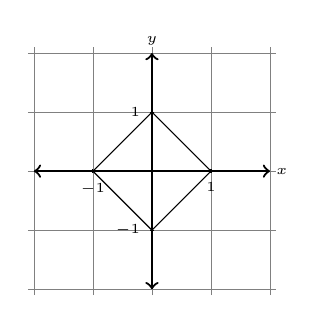
\begin{tikzpicture}[scale = 0.75]
			\draw[step=1cm,gray,very thin] (-2.1,-2.1) grid (2.1,2.1);
			\draw[thick,->] (0,0) -- (2,0);
			\draw[thick,->] (0,0) -- (0, 2);
			\draw[thick,->] (0,0) -- (-2,0);
			\draw[thick,->] (0,0) -- (0, -2);
			\node[] at (2.2, 0) {\tiny $x$};
			\node[] at (0, 2.2) {\tiny $y$};
			\foreach \x in {-1, 1}
   \draw (\x cm,1pt) -- (\x cm,-1pt) node[anchor=north] {\tiny $\x$};
\foreach \y in {-1, 1}
    \draw (1pt,\y cm) -- (-1pt,\y cm) node[anchor=east] {\tiny $\y$};

    \draw[] (1, 0) -- (0, 1) -- (-1, 0) -- (0, -1) -- cycle;

		\end{tikzpicture}
	\end{figure}
	}
	\uncover<3->{This is precisely the square given by $|x| + |y| = 1$ for $(x, y) \in \mathbb{R}^2.$ }\\
	\uncover<4->{Thus, our line integral is simply $\displaystyle\oint_Cdx+dy.$ }\\
	\uncover<5->{The above can be written as $\displaystyle\oint_C \nabla(x + y)\cdot d\mathbf{r}.$ As $C$ is a closed path, we get $0.$ }
\end{frame}
\begin{frame}{Sheet 10}
	(9) The verification of $\dfrac{\partial}{\partial y}f_1(x, y) = \dfrac{\partial}{\partial x}f_2(x, y)$ can be done easily.\\
	\uncover<2->{Now, recall that $\mathbf{F}$ is a gradient of a scalar field on $S$  } \uncover<3->{ $\iff$ line integrals of $\mathbf{F}$ are path-independent in $S$  } \uncover<4->{ $\iff$ the line integral of $\mathbf{F}$ along every closed path that lies in $S$ is zero.}\\
	\uncover<5->{We shall show that $\mathbf{F}$ is not a gradient of a scalar field on $S$ by showing that the third condition is not true. }\\
	\uncover<6->{Indeed, consider the path $\mathbf{\gamma}:[-\pi, \pi]\to\mathbb{R}^2$ given as $(\cos t, \sin t).$ }\uncover<7->{Then, $\mathbf{\gamma}$ is indeed a closed path which lies in $S.$ }\\
	\uncover<8->{Now, we compute $\displaystyle\oint_\gamma \mathbf{F}\cdot d\mathbf{s}.$ }
	\begin{align*}
		\uncover<9->{\oint_\gamma \mathbf{F}\cdot d\mathbf{s} &= \int_{-\pi}^{\pi} \sin^2t + \cos^2 t dt  }\\
		\uncover<10->{ &= \int_{-\pi}^{\pi} 1 dt  }	\uncover<11->{ = 2\pi } \uncover<12->{{\color[rgb]{1, 0, 0} \neq 0.} }
	\end{align*}
\end{frame}
\begin{frame}{Sheet 10}
	Thus, we have shown that $\mathbf{F}$ cannot be the gradient of a scalar field on $S.$\\~\\
	\uncover<2->{This shows us that curl being zero is not a sufficient condition for a field to be a gradient field. }\\
	\uncover<3->{(Technically, we can't talk about curl as this is not a 3D vector field but it can easily be extended to one with our domain then being $(\mathbb{R}\setminus\{0\})^2\times\mathbb{R} \subset \mathbb{R}^3.$)}\\
	\uncover<4->{However, later in the course, we'll see a condition on the ``geometry'' of the domain that would indeed imply that curl-free fields are grad fields. }\\~\\
	\uncover<5->{Can you think of examples of when geometry of domain affected the behaviour of functions in the case of one-variable calculus? }	
\end{frame}
\end{document}